\documentclass[tikz]{standalone}
\usepackage{amsmath}
\usepackage{amsfonts}
\usepackage{amssymb}
\usepackage{tikz}

\usetikzlibrary{decorations.pathreplacing}
\usetikzlibrary{decorations.text}
\usetikzlibrary{arrows,shapes,backgrounds, shadows,fadings, calc, positioning, intersections}
\usepackage{pagecolor,lipsum}
\usepackage{color}
\definecolor{ColorA}{HTML}{376fcc}
\definecolor{ColorB}{HTML}{bc4949}
\definecolor{ColorC}{rgb}{.4,.165,.6}
\definecolor{A}{HTML}{F9F8EB}
\definecolor{B}{HTML}{FFE1B6}
\definecolor{C}{HTML}{7A9EB1}

\usepackage[nomessages]{fp}% 

\def\Primary{{I,V,S,N,P,F,M}}

\usepackage{fontspec}
\setmainfont{Source Sans Pro}
\setmathrm{Arial}
\setmathsf{Arial}
\setmathtt{Arial}

\begin{document}

		%\pagecolor{A}
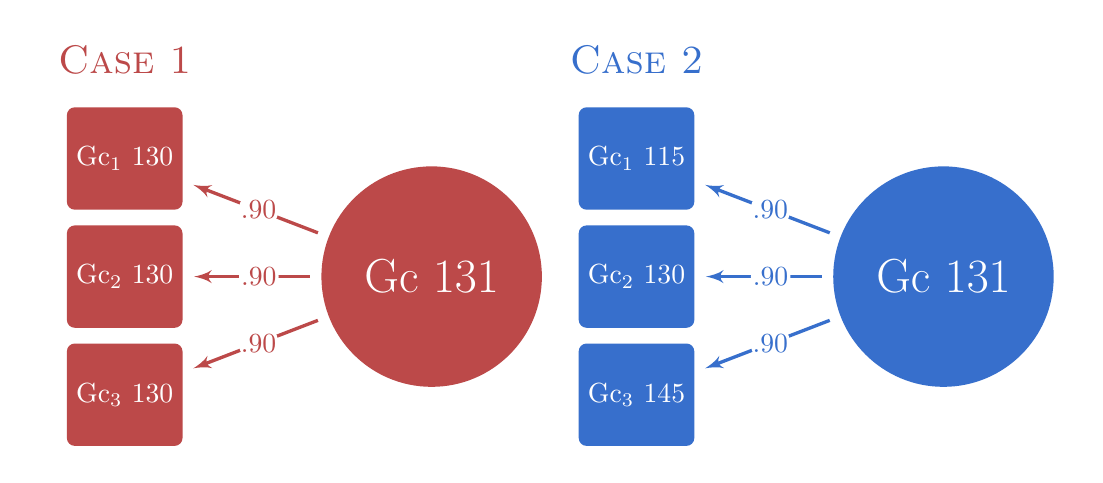
\begin{tikzpicture}[
latent/.style={
	circle,
	fill= black!30,
	minimum size=2.8cm,
	font=\LARGE,
	align=center,
	text = white},
latentlong/.style={
	circle,
	fill= black!30,
	minimum size=2.8cm,
	font=\normalsize,
	align=center,
	text = black!90},
error/.style={
	circle,
	text=black!90,
	fill = black!30,
	inner sep=0mm,
	minimum size=1cm,
	font=\large},
ob/.style={
	rectangle,
	fill=black!30,
	minimum width=1.3cm,
	align=center,
	minimum height=1.3cm,
	rounded corners = 1mm,
	font=\normalsize,
	text = white},
post/.style={
	->,
	draw,
	shorten >=4pt,
	shorten <=4pt,
	>=latex',
	very thick,
	color = black!15,
	text = black},
cov/.style={
	<->,
	shorten >=4pt,
	shorten <=4pt,
	>=latex',
	thick,
	font=\Large,
	bend left=50,
	color = black!50,
	text = black,draw},
variance/.style={
	<->,
	>=latex',
	thick,
	bend left=245,
	looseness=4.5,
	shorten >=2pt,
	shorten <=2pt,
	font=\small,
	color = black!50,
	text = black,
	draw},
label/.style={
	fill=white,
	font=\normalsize,
	circle,
%	fill = A,
	inner sep = 0mm,
	pos=.48}]


%Observed Vars

\foreach \i[count=\ii from 10] in {1,2,3}{%make ii based on i
	\node[ob, fill = black!15, fill = ColorB, text = white]  (Gc\i) at (0,-\i*1.5){Gc\textsubscript{\i} 130};
}

\node[latent, fill = black!15, right = 1.75cm of Gc2, fill = ColorB] (Gc) {Gc 131};


\path[post, color = ColorB] (Gc) to node[label]  { .90}  (Gc1);
\path[post, color = ColorB] (Gc) to node[label, pos = .45]  { .90}  (Gc2);
\path[post, color = ColorB] (Gc) to node[label]  { .90}  (Gc3);


\node[above = 0.3cm of Gc1, text = ColorB, font = \Large] (A)  {\textsc{Case 1}};

\node[ob, fill = black!15, fill = ColorA]  (Gc1) at (6.5,-1*1.5){Gc\textsubscript{1} 115};
\node[ob, fill = black!15, fill = ColorA]  (Gc2) at (6.5,-2*1.5){Gc\textsubscript{2} 130};
\node[ob, fill = black!15, fill = ColorA]  (Gc3) at (6.5,-3*1.5){Gc\textsubscript{3} 145};

\node[latent, fill = black!15, right = 1.75cm of Gc2, fill = ColorA] (Gc) {Gc 131};

\path[post, color = ColorA] (Gc) to node[label]  { .90}  (Gc1);
\path[post, color = ColorA] (Gc) to node[label, pos = .45]  { .90}  (Gc2);
\path[post, color = ColorA] (Gc) to node[label]  { .90}  (Gc3);

\node[above = 0.3cm of Gc1, text = ColorA, font = \Large] (A)  {\textsc{Case 2}};

\node[xshift = -1ex] at (current bounding box.south west){};
\node[xshift = 1ex] at (current bounding box.north east){};
	\end{tikzpicture}
\end{document}
